\subsection{Enumerative Search}
\label{sec:enumerative-search}

In the context of program synthesis, enumerative search consists of
enumerating programs by working the intrinsic structure of the program space to
guide the search. The programs can be ordered using many different program
metrics, the simplest one being program size~\cite{Alur:sygus:2013}, and pruned
by means of \todo{semantic equivalence checks}{Missing an example to explain
what I mean. Maybe add a simple example such as, how by associativity of
addition, x+y is the same as y+x. Symmetry breaking.} with respect to the
specification. Synthesizers based on enumerative search have been some of the
most effective to synthesize short programs in complex program
spaces~\cite{Gulwani2017}.

\begin{figure}
  \centering
  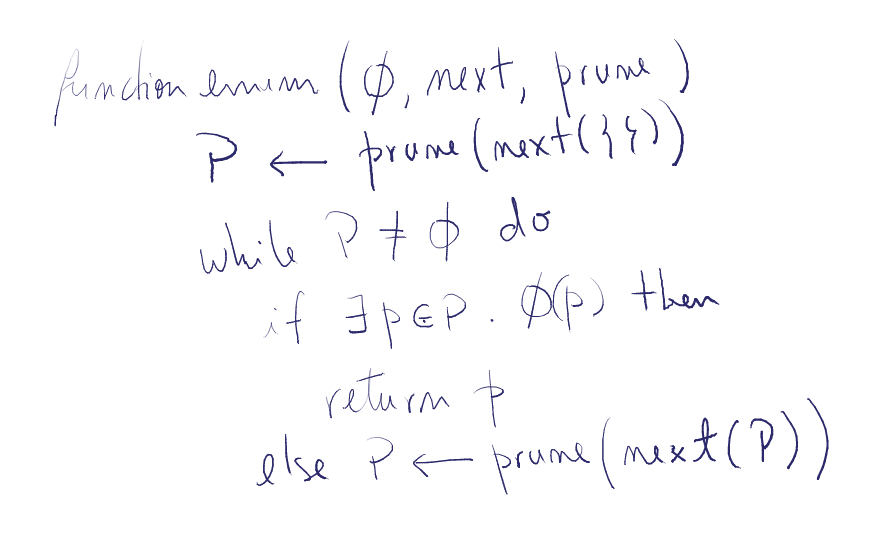
\includegraphics[width=0.5\textwidth]{assets/enum-01.png}
  \caption{FIXME: This is a placeholder.}
  \label{fig:enum-01}
\end{figure}

A simple enumerative search algorithm is described in Figure~\ref{fig:enum-01}. The
algorithm is parameterized by the specification $\phi{}$ and two procedures,
$next$, that given a set of programs generates a new set of programs, and
$prune$, that given a set of programs filters out the \todo{unwanted ones}{Isto
poderia ser dito de uma outra forma...}. The algorithm works by iteratively
calling the given procedures until it finds a program that matches the
specification.

In their overview of the field of program synthesis~\cite{Gulwani2017},
\citeauthor{Gulwani2017} \todo{present}{Professor asks if the algorithms are
  presented as original work} some simple enumerative search algorithms for
finding programs in program spaces defined by a \gls{cfg}, which we describe
next. The algorithms can be generalized to other types of program spaces such
as, e.g., partial programs.

\subsubsection{Top-Down Tree Search}
\label{sec:top-down-tree-search}

\begin{figure}
  \centering
  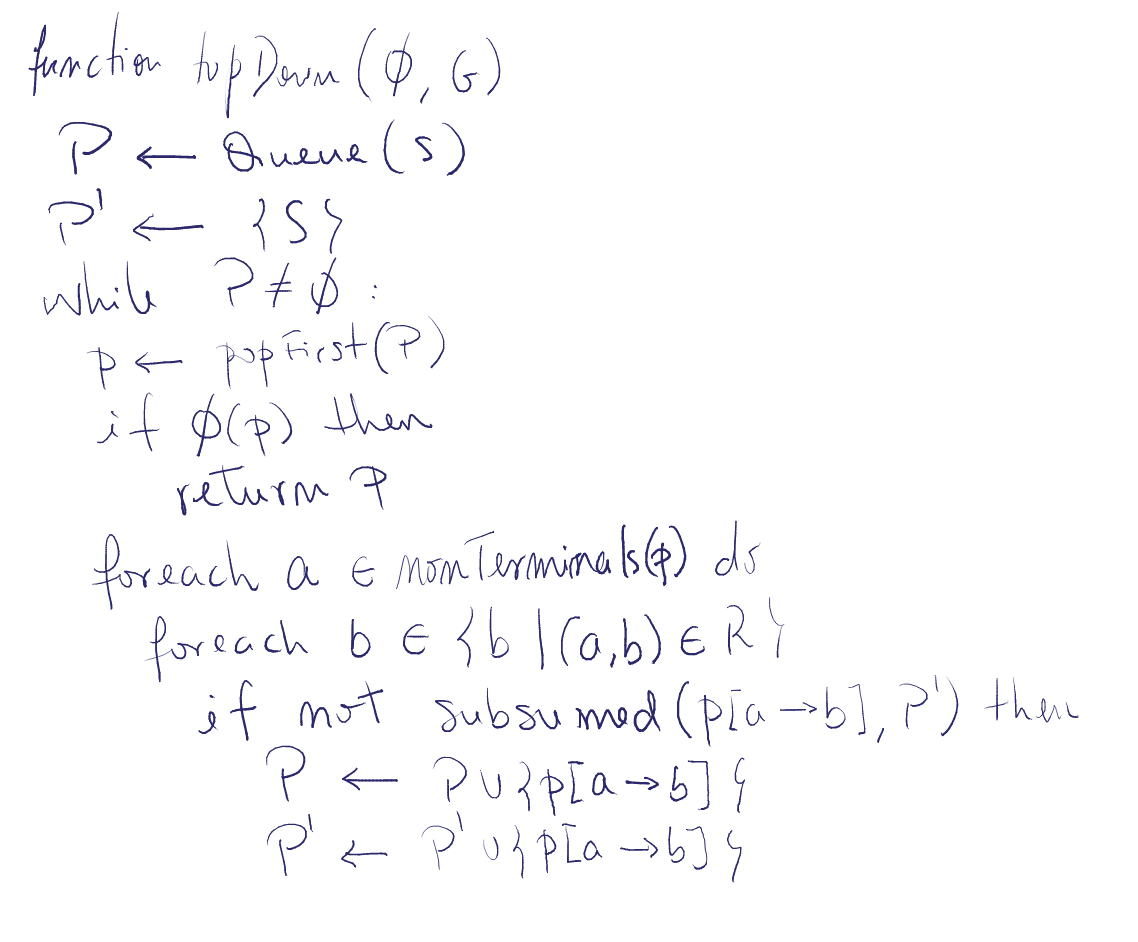
\includegraphics[width=0.5\textwidth]{assets/enum-top-down.png}
  \caption{FIXME: This is a placeholder.}
  \label{fig:enum-top-down}
\end{figure}

The first algorithm, shown in Figure~\ref{fig:enum-top-down}, takes as input a
\gls{cfg} $G = (V, \Sigma{}, R, S)$ and a specification $\phi{}$, and works by
exploring the derivations of $G$ in a best-first top-down fashion. The algorithm
stores the current programs in a priority queue, $P$, and stores all the
programs found so far in the set $P'$. Both $P$ and $P'$ are initialized with
the partial program that corresponds to the start symbol $S$ of $G$. The
algorithm runs until it finds a program $p$ that matches the specification
$\phi{}$ or there are no more programs waiting in the queue (meaning that the
algorithm fails). At every iteration, we take the program $p$ with the highest
priority from the queue and check whether it satisfies $\phi{}$. If yes, we
return $p$. Otherwise, the algorithm finds new (possibly partial) programs by
applying the production rules of the grammar to $p$. The program space is pruned
in the next step by ignoring programs that are semantically equivalent (with
respect to $\phi{}$) to programs already considered in the past ($P'$).

\subsubsection{Bottom-Up Tree Search}
\label{sec:bottom-up-tree-search}

The second algorithm, shown in Figure \fixme{?}{ainda tenho que produzir esta
figura.}, also takes a \gls{cfg} $G = (V, \Sigma{}, R, S)$ and a specification
$\phi{}$, and works by exploring the derivations of the grammar in a bottom-up
dynamic programming fashion. This strategy has the advantage over the top-down
search that (in general) only complete programs may be evaluated for semantic
equivalence. The algorithm maintains a set of semantically equivalent
expressions, first considering the programs corresponding to leafs of the syntax
tree of the grammar $G$, and then composing them in order to build expressions
of increasing complexity, essentially applying the rules of the grammar in the
opposite direction.

\subsubsection{Bidirectional Tree Search}
\label{sec:bidirectional-search}

We can see that a top-down tree search starts from a set of input states, while
a bottom-up tree search starts from a set of output states. The third algorithm,
shown in Figure \fixme{?}{ainda tenho que produzir esta figura.}, combines the
previous two approaches, starting from both a set of input states and a set of
output states. It maintains both sets, evolving in the same way the previous two
algorithms did and stopping when it finds a state that belongs to both sets in a
sort of meet-in-the-middle approach.
